%!TEX root = ../dissertation.tex

\chapter{Background}

%% FIGURE OUT HOW TO START HTIS CHAPTER HERE 
\newthought{There's something to be said} for having a good opening line. Morbi commodo, ipsum sed pharetra gravida, orci  $x = 1/\alpha$ magna rhoncus neque, id pulvinar odio lorem non turpis \cite{Eigen1971, Knuth1968}. 


\section{Causal Effects} 

A traditional understanding of causation comes from the field of medicine, where researchers can perform a controlled experiment to prove causation.  This type of study contains two sample groups, one which receives no treatment (the placebo group) and one which receives the treatment (the treatment group).  By comparing the outcome of these two groups, the researchers can demonstrate whether the outcome for patients receiving treatment differs significantly from the controls.  

To translate this idea into statistical terms, some notation must be introduced.  The random variable $A$ represents the treatment status, where a value of 1 indicates treated and a value of 0 indicates untreated.  The random variable $Y$ is the outcome variable, often with a value of 0 indicating survival and a value of 1 indicating death.  These interpretations of $A$ and $Y$ correspond to the above understanding of causation studies, but for various causal inference studies, the form of $Y$ in particular can change depending on the question of interest.  For example, $Y$ can be a continuous variable, such as the weight difference of an individual in a weight loss trial or the change in HDL levels in a cholesterol study.  

To study the causal effect of $A$, the desired value is the difference in $Y$ under varying conditions of $A$.  Notationally, this is the difference between $Y^{a=1}$, the outcome under treatment, and $Y^{a=0}$, the outcome under no treatment.  A causal effect can be seen on an individual level if $Y_i^{a=1} \neq Y_i^{a=0}$ for individual $i$.  Two difficulties arise with individual causal effects.  Firstly, statistical significance is frivolous on a sample size of one.  Furthermore, in many studies, it is impossible to have scenarios of both treatment and no treatment for the same individual, particularly if being in either group results in death.  Therefore, statisticians typically look at the average causal effect in the population, 
$$ \mathbb{E}[Y^{\; a=1}] - \mathbb{E}[Y^{\; a=0}]$$ 
Mathematically, this is equivalent to 
$$ \mathbb{E}[Y^{\; a=1} - Y^{\; a=0}]$$ 
because the average of differences is equal to the difference of averages \cite{}.  

\subsection{Assumptions} 
% Cox (1958) -- independence of observations 
% Rubin 1980 
% check textbook page 5 
%- SUTVA: http://www2.stat.duke.edu/courses/Spring14/sta320.01/Class2.pdf

	


% For an example of a full page figure, see Fig.~\ref{fig:myFullPageFigure}.


%\begin{figure}
%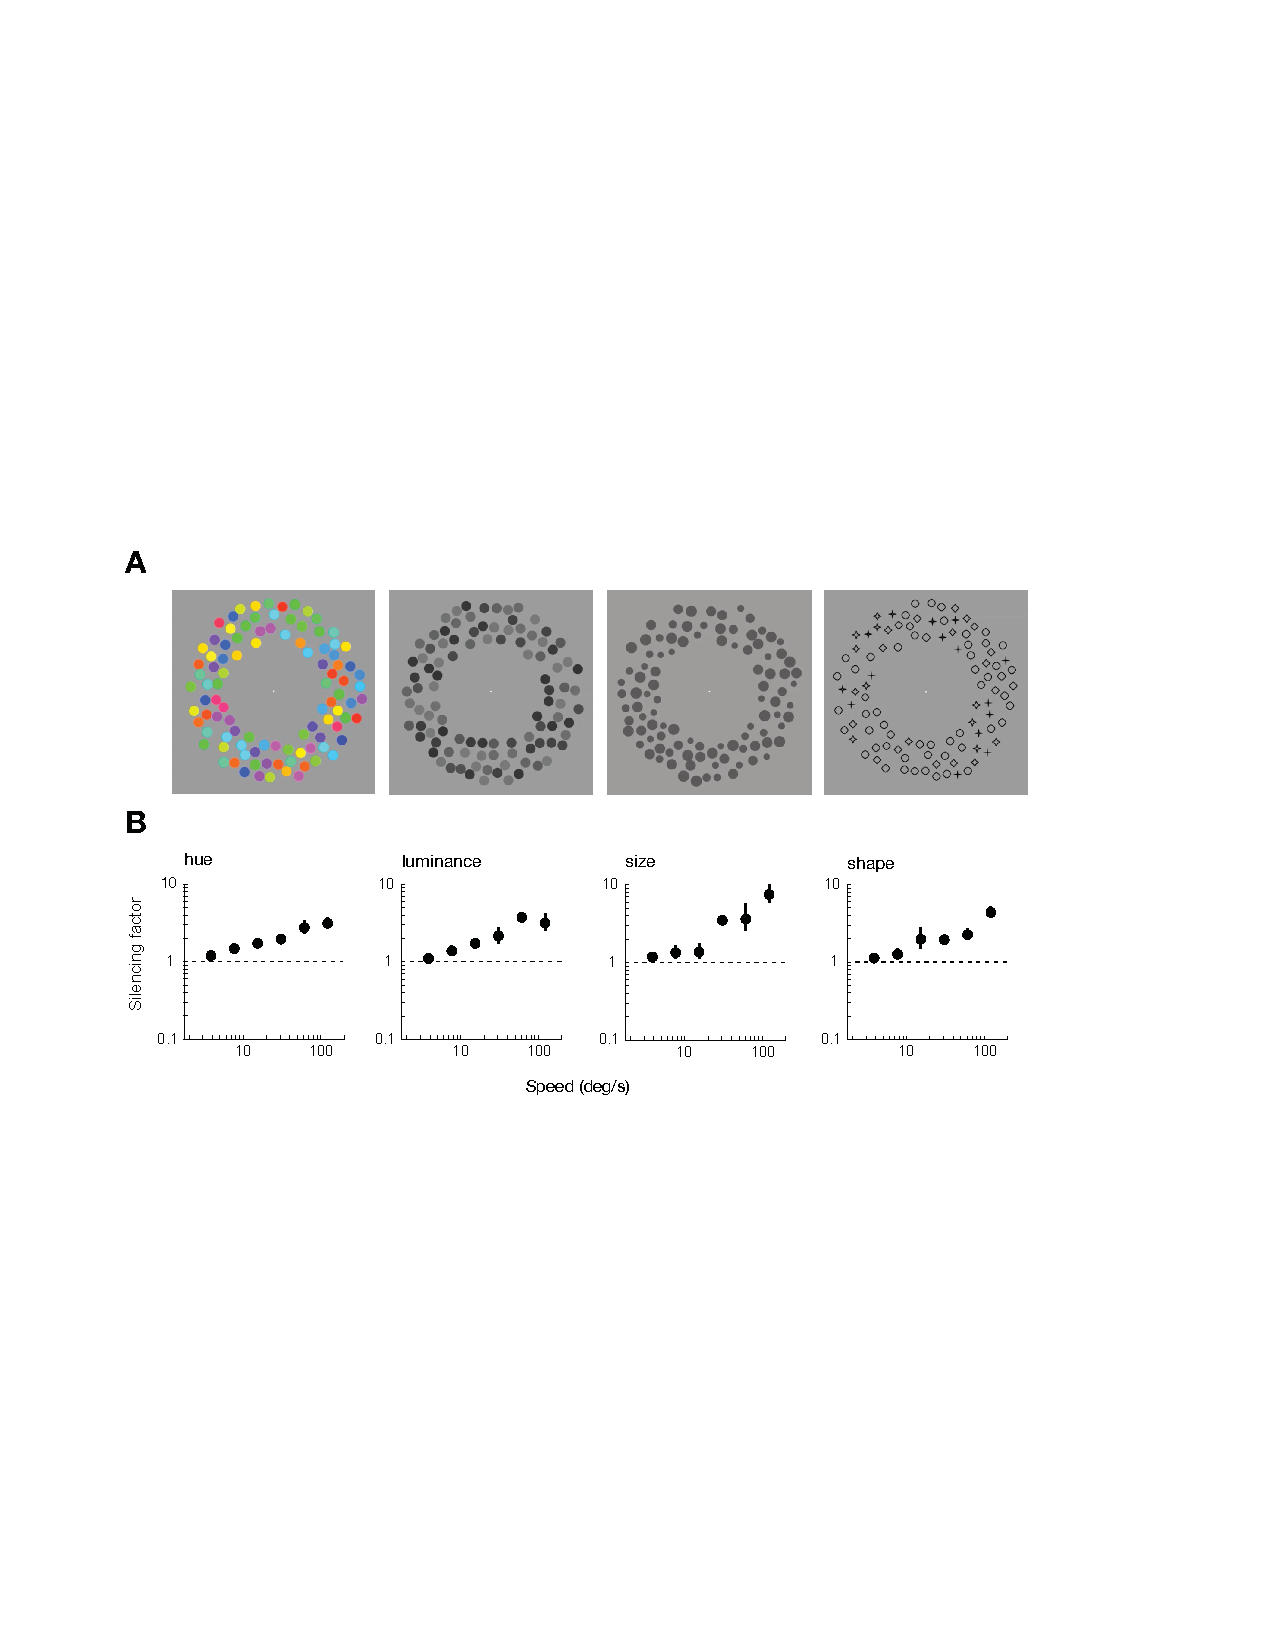
\includegraphics[width=\textwidth]{figures/fig1}
%\caption[Short figure name.]{This is a figure that floats inline and here is its caption.
%\label{fig:myInlineFigure}}
%\end{figure}
